% Created 2019-05-07 mar 21:43
% Intended LaTeX compiler: pdflatex
\documentclass[xcolor={usenames,svgnames,dvipsnames}]{beamer}
\usepackage[utf8]{inputenc}
\usepackage[T1]{fontenc}
\usepackage{graphicx}
\usepackage{grffile}
\usepackage{longtable}
\usepackage{wrapfig}
\usepackage{rotating}
\usepackage[normalem]{ulem}
\usepackage{amsmath}
\usepackage{textcomp}
\usepackage{amssymb}
\usepackage{capt-of}
\usepackage{hyperref}
\usepackage{color}
\usepackage{listings}
\usepackage{mathpazo}
\usepackage{gensymb}
\usepackage{amsmath}
\usepackage{esdiff}
\usepackage{steinmetz}
\bibliographystyle{plain}
\usepackage[emulate=units]{siunitx}
\sisetup{fraction=nice, decimalsymbol=comma, retain-unity-mantissa = false}
\newunit{\wattpeak}{Wp}
\newunit{\watthour}{Wh}
\newunit{\amperehour}{Ah}
\hypersetup{colorlinks=true, linkcolor=Blue, urlcolor=Blue}
\renewcommand{\thefootnote}{\fnsymbol{footnote}}
\beamertemplatenavigationsymbolsempty
\setbeamertemplate{footline}[frame number]
\newcommand{\laplace}[1]{\mathbf{#1}(\mathbf{s})}
\newcommand{\slp}{\mathbf{s}}
\newcommand{\fasor}[1]{\mathbf{#1}(\omega)}
\newcommand{\atan}{\mathrm{atan}}
\AtBeginSection[]{\begin{frame}[plain]\tableofcontents[currentsection,hideallsubsections]\end{frame}}
\setbeamercolor{alerted text}{fg=blue!50!black} \setbeamerfont{alerted text}{series=\bfseries}
\usetheme[hideothersubsections]{Boadilla}
\usecolortheme{rose}
\usefonttheme{serif}
\author{Oscar Perpiñán Lamigueiro}
\date{Mayo 2019}
\title{Transformadores}
\subtitle{Teoría de Circuitos II}
\hypersetup{
 pdfauthor={Oscar Perpiñán Lamigueiro},
 pdftitle={Transformadores},
 pdfkeywords={},
 pdfsubject={},
 pdfcreator={Emacs 26.1 (Org mode 9.2)}, 
 pdflang={Spanish}}
\begin{document}

\maketitle

\begin{frame}[label={sec:orgdec4f88}]{Recordatorio}
\begin{columns}
\begin{column}{0.7\columnwidth}
\begin{center}
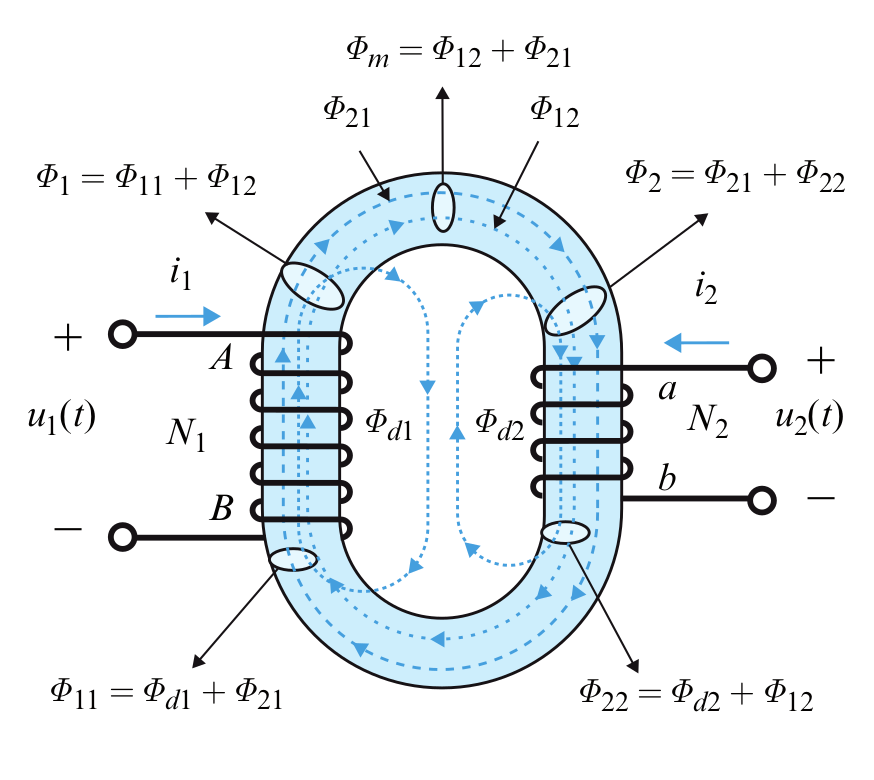
\includegraphics[width=.9\linewidth]{figs/Acoplamiento1.png}
\end{center}
\end{column}
\begin{column}{0.3\columnwidth}
\[
  L_1 = N_1 \frac{\phi_{11}}{i_1}
\]

\[
  L_2 = N_2 \frac{\phi_{22}}{i_2}
\]


\begin{align*}
  M &= N_1 \frac{\phi_{12}}{i_2}\\
    &= N_2 \frac{\phi_{21}}{i_1}
\end{align*}

\[
  M = k \sqrt{L_1 \cdot L_2}
\]
\end{column}
\end{columns}
\end{frame}

\section{Transformador Real}
\label{sec:orgc079ccb}

\begin{frame}[label={sec:orgc068016}]{Ecuaciones del Transformador Real}
\begin{center}
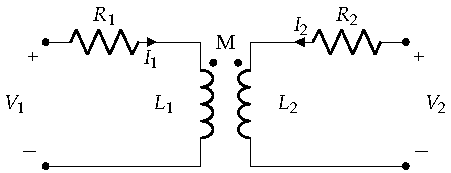
\includegraphics[height=0.45\textheight]{figs/Trafo_Real.pdf}
\end{center}

\begin{align*}
  \overline{U}_1 &= (R_1 + j \omega L_1) \cdot \overline{I}_1 + j \omega M \cdot\overline{I}_2\\
  \overline{U}_2 &= j \omega M \cdot \overline{I}_1 + (R_2 + j \omega L_2) \cdot \overline{I}_2
\end{align*}
\end{frame}

\begin{frame}[label={sec:orgc605a54}]{Ejemplo: impedancia de entrada desde primario}
\begin{center}
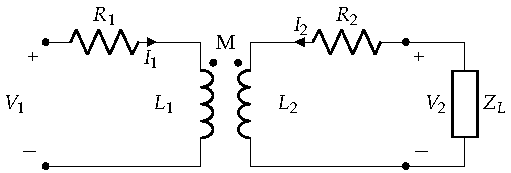
\includegraphics[height=0.45\textheight]{figs/Trafo_Real_ImpSec.pdf}
\end{center}

Ecuaciones del transformador
\begin{align*}
  \overline{U}_1 &= (R_1 + j \omega L_1) \cdot \overline{I}_1 + j \omega M \cdot\overline{I}_2\\
  \overline{U}_2 &= j \omega M \cdot \overline{I}_1 + (R_2 + j \omega L_2) \cdot \overline{I}_2
\end{align*}
Ecuación de la carga
\[
  \overline{U}_2 = - \overline{I}_2 \cdot \overline{Z}_L
\]
\end{frame}
\begin{frame}[label={sec:orgb2ac225}]{Ejemplo: impedancia de entrada desde primario}
\begin{center}
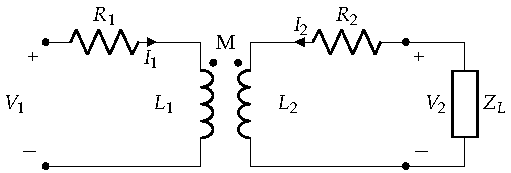
\includegraphics[height=0.45\textheight]{figs/Trafo_Real_ImpSec.pdf}
\end{center}
Combinando la ecuación del secundario con la ecuación de la carga:
\[
  \overline{I}_2  = - \frac{j \omega M}{\overline{Z}_L + (R_2 + j \omega L_2)} \cdot \overline{I}_1
\]
\end{frame}

\begin{frame}[label={sec:orgcb657e2}]{Ejemplo: impedancia de entrada desde primario}
\begin{center}
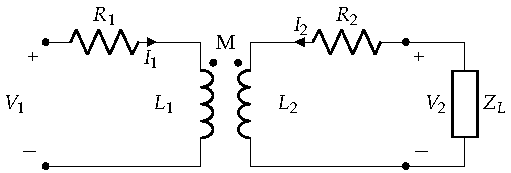
\includegraphics[height=0.45\textheight]{figs/Trafo_Real_ImpSec.pdf}
\end{center}
Combinando con la ecuación del primario:
\[
  \overline{Z}_{in}  = \frac{\overline{V}_1}{\overline{I}_1} =  (R_1 + j \omega L_1) + \frac{\omega^2 M^2}{\overline{Z}_L + (R_2 + j \omega L_2)}
\]
\end{frame}

\section{Transformador Perfecto}
\label{sec:org95a9495}
\begin{frame}[label={sec:orgf6bc4e0}]{Definición}
\begin{center}
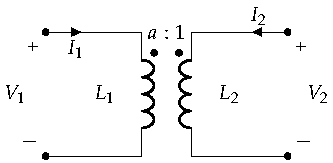
\includegraphics[height=0.35\textheight]{figs/Trafo_Perfecto.pdf}
\end{center}

Las pérdidas resistivas son despreciables.
\[
  R_1 = R_2 = 0
\]

El acoplamiento es perfecto.
\[
  k = 1
\rightarrow 
\left\{
\begin{array}{cc}
  \phi_{12} &= \phi_{22}\\
  \phi_{21} &= \phi_{11}\\
\end{array} \right.
\]
\end{frame}
\begin{frame}[label={sec:orge68ed92}]{Relación de Transformación}
Retomamos las ecuaciones de \(M_{12} = M_{21} = M\):
\[
  N_1 \frac{\phi_{12}}{i_2} = N_2 \frac{\phi_{21}}{i_1}
\]

Con la condición \(k=1\) escribimos:
\[  
  N_1 \frac{\phi_{22}}{i_2} = N_2 \frac{\phi_{11}}{i_1}
\]

Y con las definiciones de \(L_1\) y \(L_2\):
\[
  N_1 \frac{L_2}{N_2} = N_2 \frac{L_1}{N_1}
\]

Obtenemos la relación de transformación:
\[
  \boxed{\frac{L_1}{L_2} = \left(\frac{N_1}{N_2}\right)^2 = a^2}
\]
\end{frame}
\begin{frame}[label={sec:orgc9329b0}]{Ecuaciones del Transformador Perfecto}
\begin{center}
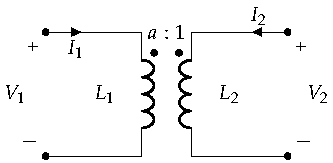
\includegraphics[height=0.45\textheight]{figs/Trafo_Perfecto.pdf}
\end{center}

\begin{align*}
  \overline{U}_1 &= j \omega L_1 \cdot \overline{I}_1 + j \omega M \cdot \overline{I}_2\\
  \overline{U}_2 &= j \omega M \cdot \overline{I}_1 + j \omega L_2 \cdot \overline{I}_2
\end{align*}
\end{frame}
\begin{frame}[label={sec:org933d811}]{Relación de Tensiones}
Dividiendo las ecuaciones:
\[
  \frac{\overline{U}_1}{\overline{U}_2} = \frac{j \omega L_1 \cdot \overline{I}_1 + j \omega M \cdot \overline{I}_2}{j \omega M \cdot \overline{I}_1 + j \omega L_2 \cdot \overline{I}_2}
\]
Empleando la relación de transformación:
\[
  \frac{L_1}{L_2} = a^2
  \rightarrow
  \left\{
  \begin{array}{ll}
    L_1 &= a^2 \cdot L_2\\
    M &= a \cdot L_2\\
  \end{array}\right.
\]
Obtenemos:
\[
  \frac{\overline{U}_1}{\overline{U}_2} = \frac{a^2 L_2 \cdot \overline{I}_1 + a L_2 \cdot \overline{I}_2}{a L_2 \cdot \overline{I}_1 + L_2 \cdot \overline{I}_2}
\]

\[
  \boxed{\frac{\overline{U}_1}{\overline{U}_2} = a = \frac{N_1}{N_2}}
\]
\end{frame}
\begin{frame}[label={sec:org9ca8fe8}]{Ejemplo: Impedancia de Entrada}
\begin{center}
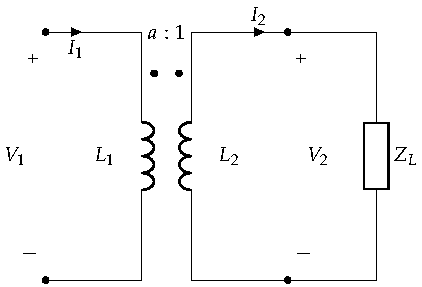
\includegraphics[height=0.45\textheight]{figs/TrafoPerfecto_ImpedanciaSecundario.pdf}
\end{center}

Ecuaciones del transformador:
\begin{align*}
  \overline{U}_1 &= j \omega L_1 \cdot \overline{I}_1 - j \omega M \cdot \overline{I}_2\\
  \overline{U}_2 &= j \omega M \cdot \overline{I}_1 - j \omega L_2 \cdot \overline{I}_2
\end{align*}
Ecuación de la impedancia:
\[
  \overline{U}_2 = \overline{Z}_L \cdot \overline{I}_2
\]
\end{frame}
\begin{frame}[label={sec:org8d0d838}]{Ejemplo: Impedancia de Entrada}
\begin{center}
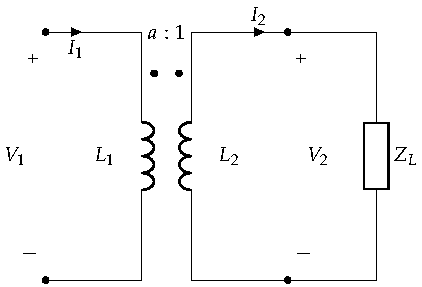
\includegraphics[height=0.45\textheight]{figs/TrafoPerfecto_ImpedanciaSecundario.pdf}
\end{center}
Despejamos \(I_2\):
\[
  \overline{I}_2 = \frac{j \omega M}{j\omega L_2 + \overline{Z}_L} \cdot \overline{I}_1
\]
Y sustituimos:
\[
  \overline{Z}_{in} = \frac{\overline{U}_1}{\overline{I}_1} = j\omega L_1 + \frac{j \omega M}{j\omega L_2 + \overline{Z}_L}
\]
\end{frame}
\begin{frame}[label={sec:orge7b54b6}]{Ejemplo: Impedancia de Entrada}
\begin{center}
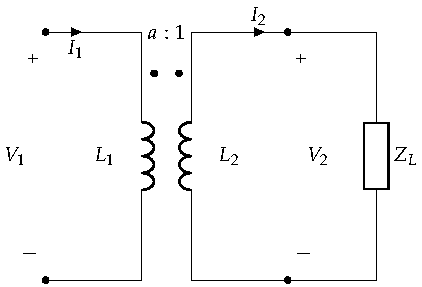
\includegraphics[height=0.45\textheight]{figs/TrafoPerfecto_ImpedanciaSecundario.pdf}
\end{center}

Teniendo en cuenta la relación entre \(L_1\), \(L_2\) y \(M\):
\[
  \boxed{\overline{Z}_{in} = \frac{j \omega L_1 \cdot (a^2 \overline{Z}_L)}{j\omega L_1 + (a^2 \cdot \overline{Z}_L)}}
\]

\[
  \boxed{\overline{Z}_{in} = a^2 \cdot \frac{j \omega L_2 \cdot \overline{Z}_L}{j\omega L_2 + \overline{Z}_L}}
\]
\end{frame}
\begin{frame}[label={sec:org962a332}]{Ejemplo: Equivalente de Thévenin desde secundario}
\begin{center}
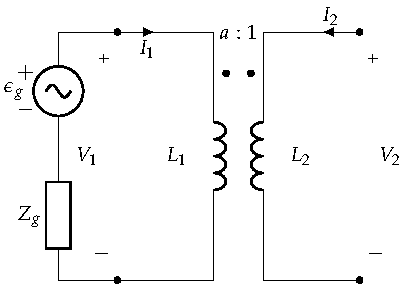
\includegraphics[width=.9\linewidth]{figs/Trafo_Perfecto_FuentePrimario.pdf}
\end{center}
\end{frame}
\begin{frame}[label={sec:orgcc8429b}]{Tensión de Thévenin}
\begin{columns}
\begin{column}{0.4\columnwidth}
\begin{center}
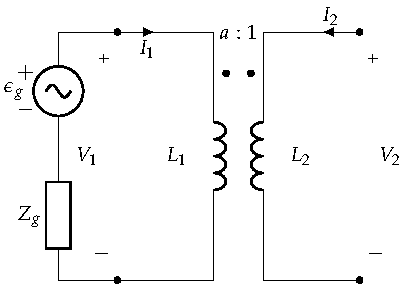
\includegraphics[width=.9\linewidth]{figs/Trafo_Perfecto_FuentePrimario.pdf}
\end{center}
\end{column}
\begin{column}{0.6\columnwidth}
Ecuaciones del transformador:
\[
  \overline{I}_2 = 0
  \rightarrow
  \left\{
    \begin{array}{ll}
      \overline{U}_1 &= j \omega L_1 \cdot \overline{I}_1\\
      \overline{U}_2 &= j \omega M \cdot \overline{I}_1\\
    \end{array}\right.
\]
Ecuación del generador:
\[
  \overline{U}_1 = \overline{\epsilon}_g - \overline{I}_1 \cdot \overline{Z}_g
\]
Tensión en abierto:
\[
  \overline{\epsilon}_{th} = \frac{j\omega M}{j\omega L_1 + \overline{Z}_g} \cdot \overline{\epsilon}_g
\]
Teniendo en cuenta que \(M = L_1/a\):
\[
  \overline{\epsilon}_{th} = \frac{1}{a} \cdot \left(\frac{j\omega L_1}{j\omega L_1 + \overline{Z}_g}\right) \cdot \overline{\epsilon}_g
\]
\end{column}
\end{columns}
\end{frame}
\begin{frame}[label={sec:org58da8ce}]{Impedancia de Thévenin}
\begin{center}
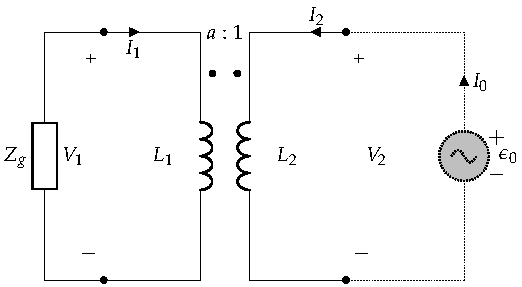
\includegraphics[width=.9\linewidth]{figs/Trafo_Perfecto_ImpedanciaPrimario.pdf}
\end{center}
\end{frame}
\begin{frame}[label={sec:org91a9d47}]{Impedancia de Thévenin}
\begin{columns}
\begin{column}{0.4\columnwidth}
\begin{center}
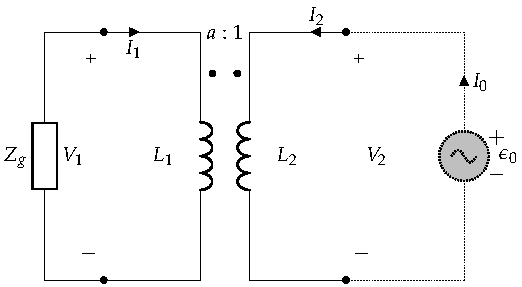
\includegraphics[width=.9\linewidth]{figs/Trafo_Perfecto_ImpedanciaPrimario.pdf}
\end{center}
\end{column}
\begin{column}{0.6\columnwidth}
Ecuaciones del transformador:
\begin{align*}
  \overline{U}_1 &= j \omega L_1 \cdot \overline{I}_1 + j \omega M \cdot\overline{I}_0\\
  \overline{\epsilon}_0 &= j \omega M \cdot \overline{I}_1 + j \omega L_2 \cdot \overline{I}_0
\end{align*}
Ecuación de la impedancia:
\[
  \overline{U}_1 = - \overline{Z}_g \cdot \overline{I}_1
\]
Impedancia de Thévenin:
\[
  \overline{Z}_{th} = \frac{\overline{\epsilon}_0}{\overline{I}_0} = j\omega L_2 + \frac{\omega^2 M^2}{j\omega L_1 + \overline{Z}_g}
\]
Con \(L_2 = L_1/a^2\) y \(M = L_1/a\):
\[
  \overline{Z}_{th} = \frac{1}{a^2} \cdot \frac{j \omega L_1 \cdot \overline{Z}_g}{j\omega L_1 + \overline{Z}_g}
\]
\end{column}
\end{columns}
\end{frame}
\begin{frame}[label={sec:orgb6da8ca}]{Resumen: Equivalente de Thévenin}
\begin{center}
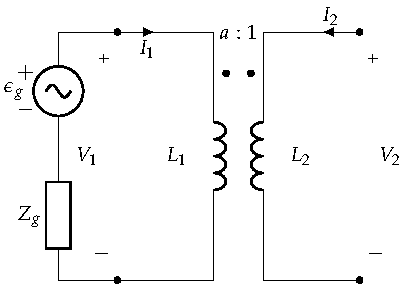
\includegraphics[height=0.5\textheight]{figs/Trafo_Perfecto_FuentePrimario.pdf}
\end{center}

\[
  \overline{Z}_{th} = \frac{1}{a^2} \cdot \frac{j \omega L_1 \cdot \overline{Z}_g}{j\omega L_1 + \overline{Z}_g}
\]

\[
  \overline{\epsilon}_{th} = \frac{1}{a} \cdot \left(\frac{j\omega L_1}{j\omega L_1 + \overline{Z}_g}\right) \cdot \overline{\epsilon}_g
\]
\end{frame}


\section{Transformador Ideal}
\label{sec:orgd188875}
\begin{frame}[label={sec:orgc0b1cf1}]{Definición}
\begin{center}
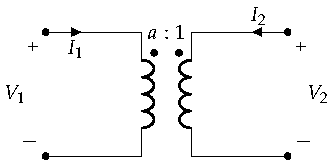
\includegraphics[height=0.35\textheight]{figs/Trafo_Ideal.pdf}
\end{center}

Las pérdidas resistivas son despreciables.
\[
  R_1 = R_2 = 0
\]

El acoplamiento es perfecto.
\[
  k = 1
\]

Las bobinas tienen un número muy elevado de espiras.

\begin{align*}
  N_1 &\to \infty\\
  N_2 &\to \infty
\end{align*}
\end{frame}
\begin{frame}[label={sec:org56961e6}]{El flujo en cada bobina es nulo}
Para que las tensiones inducidas sean finitas\ldots{} 

\begin{align*}
  \overline{U}_1 &= N_1 \overline{\phi}_1\\ 
  \overline{U}_2 &= N_2 \overline{\phi}_2
\end{align*}
\ldots{}los flujos (fasoriales) que los atraviesan deben ser nulos.
\begin{align*}
  \overline{\phi}_1 &\to 0\\
  \overline{\phi}_2 &\to 0\\
\end{align*}
Siendo:
\begin{align*}
  \overline{\phi}_1 &= \overline{\phi}_{11} + \overline{\phi}_{12}\\
  \overline{\phi}_2 &= \overline{\phi}_{22} + \overline{\phi}_{21}
\end{align*}
\end{frame}
\begin{frame}[label={sec:org9df338c}]{El flujo mutuo es nulo}
Teniendo en cuenta que el acoplamiento es perfecto, \(k = 1\):
\[
  \left.
    \begin{array}{ll}
      \phi_{12} &= \phi_{22}\\
      \phi_{21} &= \phi_{11}\\
    \end{array} \right\} 
  \rightarrow
  \left\{
    \begin{array}{ll}
      0 &= \overline{\phi}_{21} + \overline{\phi}_{12}\\
      0 &= \overline{\phi}_{12} + \overline{\phi}_{21}\\
    \end{array}\right.
\]

O también:

\[
  \boxed{\overline{\phi}_{11} + \overline{\phi}_{22} = 0}
\]
\end{frame}
\begin{frame}[label={sec:orge8b9149}]{Relación de Transformación}
Hemos obtenido:
\[
  \overline{\phi}_{11} + \overline{\phi}_{22} = 0
\]

Con las definiciones de \(L_1\), \(L_2\):
\[
  L_1 = N_1 \frac{\phi_{11}}{I_1}; \quad L_2 = N_2 \frac{\phi_{22}}{I_2}
\]
Podemos escribir:
\[
  \frac{L_1 \overline{I}_1}{N_1} + \frac{L_2 \overline{I}_2}{N_2} = 0
\]
Y con la relación entre ambas obtenemos
\[
  L_1 = L_2 \cdot \left(\frac{N_1}{N_2}\right)^2
  \rightarrow
  \frac{N_1L_2 \overline{I}_1}{N^2_2} + \frac{L_2 \overline{I}_2}{N_2} = 0
  \rightarrow
  \boxed{\frac{\overline{I}_1}{\overline{I}_2} = \mp \frac{1}{a} = \mp \frac{N_2}{N_1}}
\]
\end{frame}
\begin{frame}[label={sec:orgeffb330}]{Un transformador ideal no consume potencia}
\[
  \overline{S}_1 = \overline{V}_1 \cdot \overline{I}_1^*
\]

\[
  \overline{S}_2 = \overline{V}_2 \cdot \overline{I}_2^* 
\]

\[
  \overline{V}_2 \cdot \overline{I}_2^* = \frac{1}{a} \cdot \overline{V}_1 \cdot a \cdot \overline{I}_1^* = \overline{S}_1
\]

\[
  \boxed{\overline{S}_1 = \overline{S}_2}
  \quad
  \boxed{P_1 = P_2}
  \quad
  \boxed{Q_1 = Q_2}
\]
\end{frame}
\section{Transferencia de Circuitos}
\label{sec:orge19d3d9}
\begin{frame}[label={sec:orgb01253f}]{Fuente de Tensión de Secundario a Primario}
\begin{center}
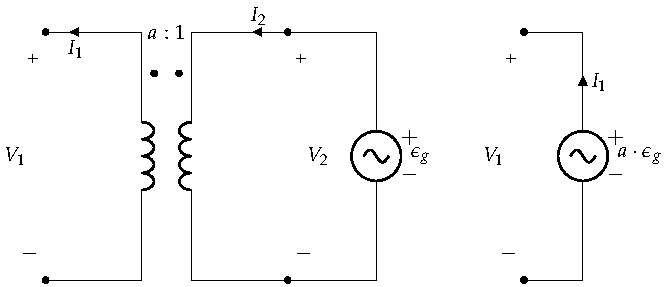
\includegraphics[width=.9\linewidth]{figs/TrafoIdeal_VSec.pdf}
\end{center}

\[
  \overline{V}_1 = a \cdot \overline{V}_2 \rightarrow \boxed{\overline{\epsilon}_{g1} = a \cdot \overline{\epsilon}_g}
\]
\end{frame}
\begin{frame}[label={sec:orgc0f2aec}]{Fuente de Tensión de Primario a Secundario}
\begin{center}
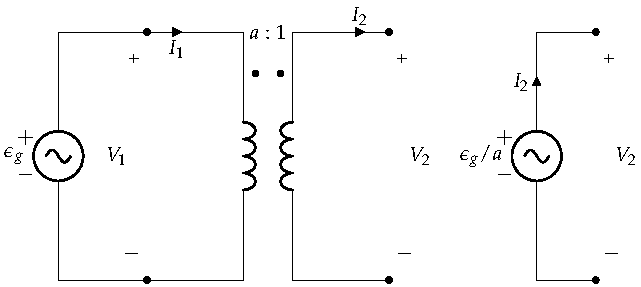
\includegraphics[width=.9\linewidth]{figs/TrafoIdeal_VPrim.pdf}
\end{center}

\[
  \overline{V}_2 = \overline{V}_1 / a \rightarrow \boxed{\overline{\epsilon}_{g2} = \overline{\epsilon}_g / a}
\]
\end{frame}
\begin{frame}[label={sec:org361efd4}]{Fuente de Corriente de Secundario a Primario}
\begin{center}
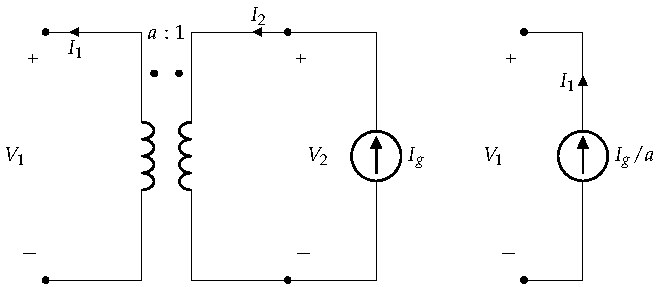
\includegraphics[width=.9\linewidth]{figs/TrafoIdeal_ISec.pdf}
\end{center}

\[
  \overline{I}_1 = \overline{I}_2 / a \rightarrow \boxed{\overline{I}_{g1} = \overline{I}_g / a} 
\]
\end{frame}
\begin{frame}[label={sec:org1140e9c}]{Fuente de Corriente de Primario a Secundario}
\begin{center}
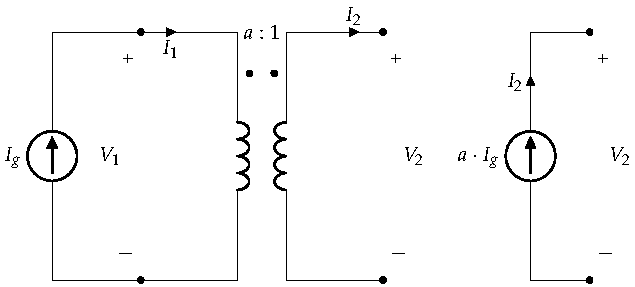
\includegraphics[width=.9\linewidth]{figs/TrafoIdeal_IPrim.pdf}
\end{center}

\[
  \overline{I}_2 = a \cdot \overline{I}_1 \rightarrow \boxed{\overline{I}_{g2} = a \cdot \overline{I}_g}
\]
\end{frame}
\begin{frame}[label={sec:org6a81459}]{Impedancia de Secundario a Primario}
\begin{center}
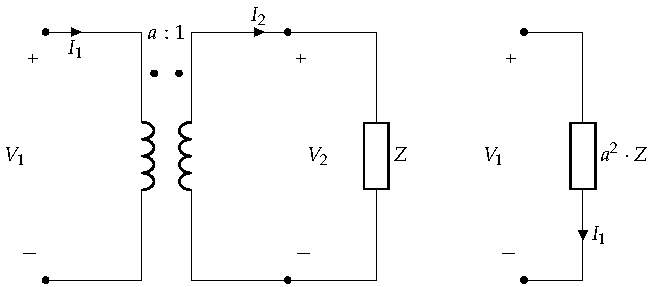
\includegraphics[width=.9\linewidth]{figs/TrafoIdeal_ZSec.pdf}
\end{center}

\[
  \left.
    \begin{array}{ll}
    \overline{V}_1 &= a \cdot \overline{V}_2\\
    \overline{I}_1 &= \overline{I}_2 / a\\
  \end{array}\right\}
   \rightarrow \boxed{\overline{Z}_1 = \frac{\overline{V}_1}{\overline{I}_1} = a^2 \cdot \overline{Z}} 
\]
\end{frame}
\begin{frame}[label={sec:org6f9a461}]{Impedancia de Primario a Secundario}
\begin{center}
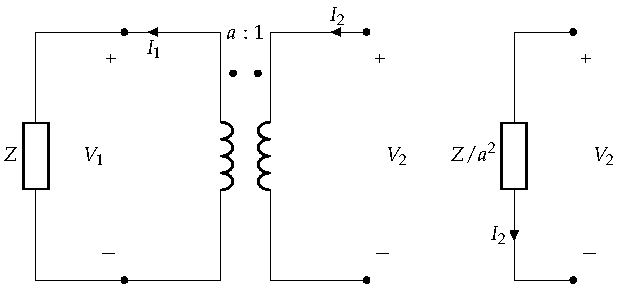
\includegraphics[width=.9\linewidth]{figs/TrafoIdeal_ZPrim.pdf}
\end{center}

\[
  \left.
    \begin{array}{ll}
    \overline{V}_2 &= \overline{V}_1 /a\\
    \overline{I}_2 &= a \cdot \overline{I}_1\\
  \end{array}\right\}
   \rightarrow \boxed{\overline{Z}_2 = \frac{\overline{V}_2}{\overline{I}_2} = \overline{Z} / a^2} 
\]
\end{frame}
\section{Transformador Perfecto vs. Transformador Ideal}
\label{sec:orgfc0e37d}
\begin{frame}[label={sec:orgad0c699}]{Recordatorio: impedancia de entrada de un T. Perfecto}
\begin{center}
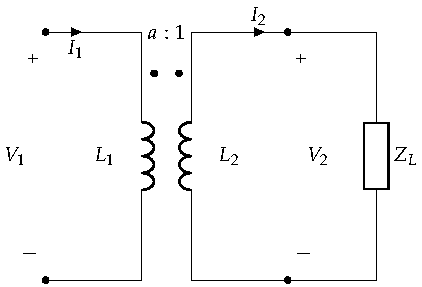
\includegraphics[height=0.45\textheight]{figs/TrafoPerfecto_ImpedanciaSecundario.pdf}
\end{center}

\[
  \boxed{\overline{Z}_{in} = \frac{j \omega L_1 \cdot (a^2 \overline{Z}_L)}{j\omega L_1 + (a^2 \cdot \overline{Z}_L)}}
\]

\[
  \boxed{\overline{Z}_{in} = a^2 \cdot \frac{j \omega L_2 \cdot \overline{Z}_L}{j\omega L_2 + \overline{Z}_L}}
\]
\end{frame}
\begin{frame}[label={sec:org54cf8a2}]{Circuito equivalente con transformador ideal}
\begin{columns}
\begin{column}{0.5\columnwidth}
\begin{center}
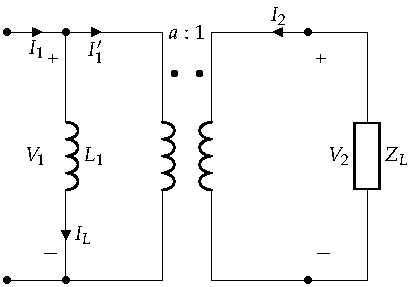
\includegraphics[width=.9\linewidth]{figs/TrafoPerfecto_Ideal.pdf}
\end{center}

\[
  \boxed{\overline{Z}_{in} = \frac{j \omega L_1 \cdot (a^2 \overline{Z}_L)}{j\omega L_1 + (a^2 \cdot \overline{Z}_L)}}
\]
\end{column}
\begin{column}{0.5\columnwidth}
\begin{center}
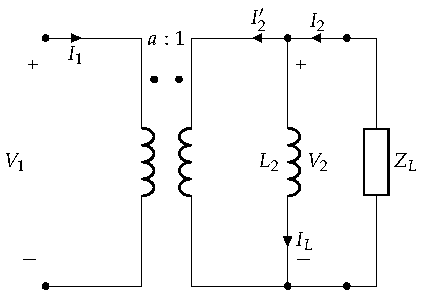
\includegraphics[width=.9\linewidth]{figs/TrafoPerfecto_Ideal2.pdf}
\end{center}

\[
  \boxed{\overline{Z}_{in} = a^2 \cdot \frac{j \omega L_2 \cdot \overline{Z}_L}{j\omega L_2 + \overline{Z}_L}}
\]
\end{column}
\end{columns}
\end{frame}

\begin{frame}[label={sec:org39a62a1}]{Recordatorio: Equivalente de Thévenin}
\begin{center}
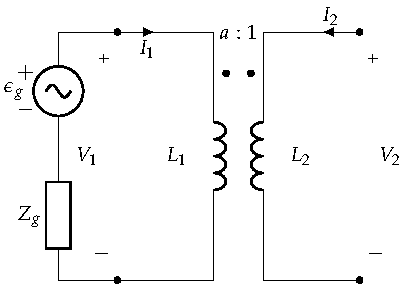
\includegraphics[height=0.5\textheight]{figs/Trafo_Perfecto_FuentePrimario.pdf}
\end{center}

\[
  \overline{Z}_{th} = \frac{1}{a^2} \cdot \frac{j \omega L_1 \cdot \overline{Z}_g}{j\omega L_1 + \overline{Z}_g}
\]

\[
  \overline{\epsilon}_{th} = \frac{1}{a} \cdot \left(\frac{j\omega L_1}{j\omega L_1 + \overline{Z}_g}\right) \cdot \overline{\epsilon}_g
\]
\end{frame}

\begin{frame}[label={sec:org5575a21}]{Equivalente en primario con transformador ideal}
\[
  \overline{Z}_{th} = \frac{1}{a^2} \cdot \frac{j \omega L_1 \cdot \overline{Z}_g}{j\omega L_1 + \overline{Z}_g}
\]

\[
  \overline{\epsilon}_{th} = \frac{1}{a} \cdot \left(\frac{j\omega L_1}{j\omega L_1 + \overline{Z}_g}\right) \cdot \overline{\epsilon}_g
\]

\begin{center}
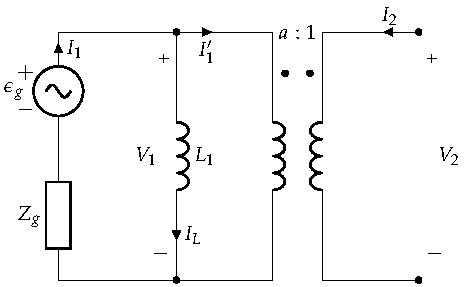
\includegraphics[height=0.5\textheight]{figs/TrafoPerfecto_Ideal_FuentePrim.pdf}
\end{center}
\end{frame}
\begin{frame}[label={sec:org3c4df0d}]{Equivalente en secundario con transformador ideal}
\[
  \overline{Z}_{th} = a^2 \cdot \frac{j \omega L_2 \cdot \overline{Z}_g}{j\omega L_2 + \overline{Z}_g}
\]

\[
  \overline{\epsilon}_{th} = a \cdot \left(\frac{j\omega L_2}{j\omega L_2 + \overline{Z}_g}\right) \cdot \overline{\epsilon}_g
\]

\begin{center}
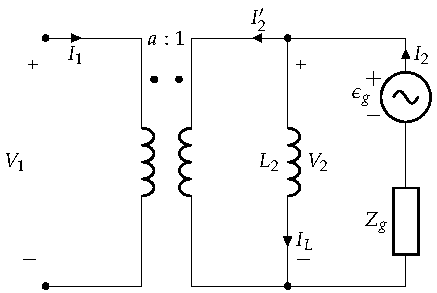
\includegraphics[height=0.5\textheight]{figs/TrafoPerfecto_Ideal_FuenteSec.pdf}
\end{center}
\end{frame}
\section{Transformador de Varios Devanados}
\label{sec:orgb428816}
\begin{frame}[label={sec:org42eee8f}]{Transformador Real de Varios Devanados}
\begin{center}
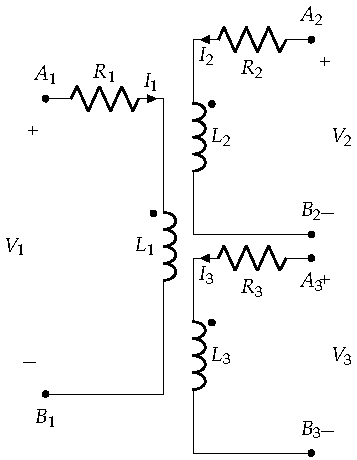
\includegraphics[height=0.9\textheight]{figs/TrafoVariosDevanados.pdf}
\end{center}
\end{frame}

\begin{frame}[label={sec:org36d9744}]{Ecuaciones del Transformador Real}
\begin{center}
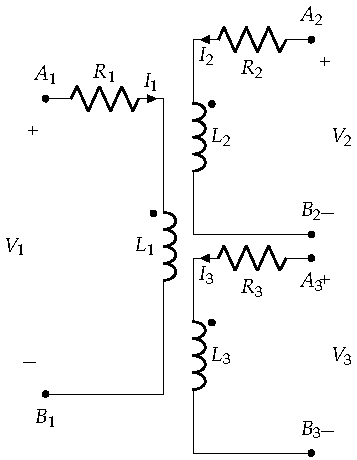
\includegraphics[height=0.6\textheight]{figs/TrafoVariosDevanados.pdf}
\end{center}

\begin{align*}
  \overline{U}_1 &= (R_1 + j \omega L_1) \cdot \overline{I}_1 + j \omega M_{12} \cdot\overline{I}_2 + j \omega M_{13} \cdot\overline{I}_3\\
  \overline{U}_2 &= j \omega M_{12} \cdot \overline{I}_1 + (R_2 + j \omega L_2) \cdot \overline{I}_2 + j \omega M_{23} \cdot \overline{I}_3\\
  \overline{U}_3 &= j \omega M_{13} \cdot \overline{I}_1 + j \omega M_{12} \cdot\overline{I}_2 + (R_3 + j \omega L_3) \cdot \overline{I}_3
\end{align*}
\end{frame}

\begin{frame}[label={sec:org7860964}]{Transformador Perfecto}
\begin{columns}
\begin{column}{0.6\columnwidth}
\begin{center}
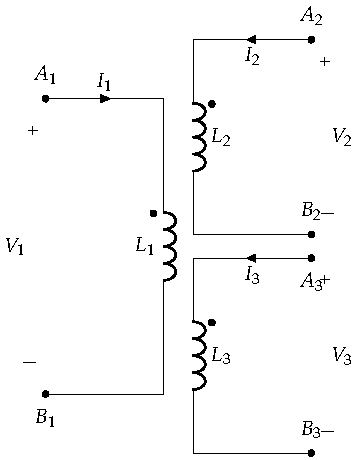
\includegraphics[height=0.8\textheight]{figs/TrafoPerfectoVariosDevanados.pdf}
\end{center}
\end{column}

\begin{column}{0.4\columnwidth}
Las pérdidas resistivas son despreciables.
\[
  R_1 = R_2 = R_3 = 0
\]

El acoplamiento es perfecto.
\[
  k_{12} = k_{13} = k_{23} = 1
\]
\end{column}
\end{columns}
\end{frame}

\begin{frame}[label={sec:org69ec244}]{Ecuaciones del Transformador Perfecto}
\begin{center}
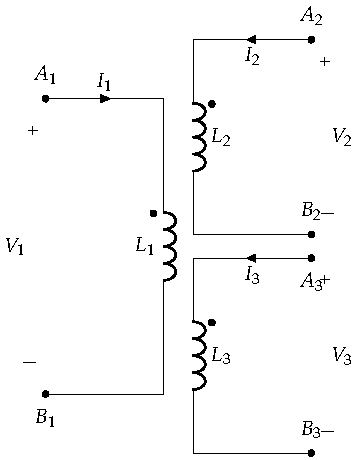
\includegraphics[height=0.6\textheight]{figs/TrafoPerfectoVariosDevanados.pdf}
\end{center}

\begin{align*}
  \overline{U}_1 &= j \omega L_1 \cdot \overline{I}_1 + j \omega M_{12} \cdot\overline{I}_2 + j \omega M_{13} \cdot\overline{I}_3\\
  \overline{U}_2 &= j \omega M_{12} \cdot \overline{I}_1 + j \omega L_2 \cdot \overline{I}_2 + j \omega M_{23} \cdot \overline{I}_3\\
  \overline{U}_3 &= j \omega M_{13} \cdot \overline{I}_1 + j \omega M_{12} \cdot\overline{I}_2 + j \omega L_3 \cdot \overline{I}_3
\end{align*}
\end{frame}

\begin{frame}[label={sec:orgf35a579}]{Relaciones de Transformación}
\begin{columns}
\begin{column}{0.6\columnwidth}
\begin{center}
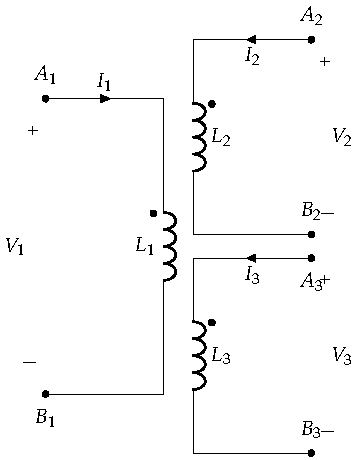
\includegraphics[height=0.6\textheight]{figs/TrafoPerfectoVariosDevanados.pdf}
\end{center}
\end{column}

\begin{column}{0.4\columnwidth}
\begin{align*}
  \frac{L_1}{L_2} &= \left(\frac{N_1}{N_2}\right)^2 = a^2_{12}\\
  \frac{L_1}{L_3} &= \left(\frac{N_1}{N_3}\right)^2 = a^2_{13}
\end{align*}

\begin{align*}
  \frac{\overline{U}_1}{\overline{U}_2} &= a_{12}\\
  \frac{\overline{U}_1}{\overline{U}_3} &= a_{13}
\end{align*}
\end{column}
\end{columns}
\end{frame}

\begin{frame}[label={sec:orgc630a92}]{Transformador Ideal}
\begin{center}
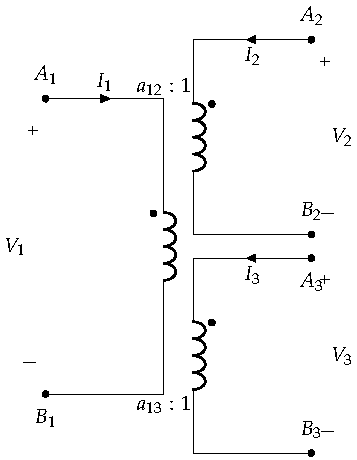
\includegraphics[height=0.9\textheight]{figs/TrafoIdealVariosDevanados.pdf}
\end{center}
\end{frame}

\begin{frame}[label={sec:org39608ba}]{Relación de Transformación del Transformador Ideal}
\begin{center}
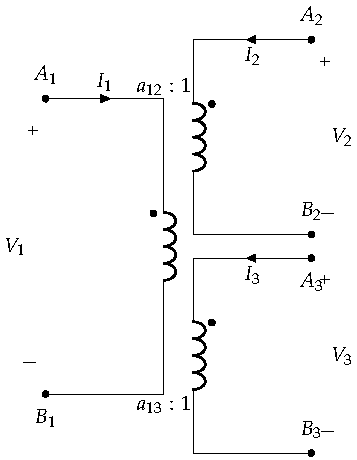
\includegraphics[height=0.45\textheight]{figs/TrafoIdealVariosDevanados.pdf}
\end{center}

Debido a las condiciones de idealidad:

\[
  \overline{\phi}_{11} \pm \overline{\phi}_{22} \pm \overline{\phi}_{33} = 0
\]

\[
  N_1 \overline{I}_1 \pm N_ 2\overline{I}_2 \pm N_3 \overline{I}_{3} = 0
\]

En términos de corriente:
\[
  \boxed{\overline{I}_1 = \mp 1/a_{12} \cdot \overline{I}_2 \mp 1/a_{13} \cdot  \overline{I}_3}
\]
\end{frame}

\begin{frame}[label={sec:org054798d}]{Impedancia de Entrada}
\begin{center}
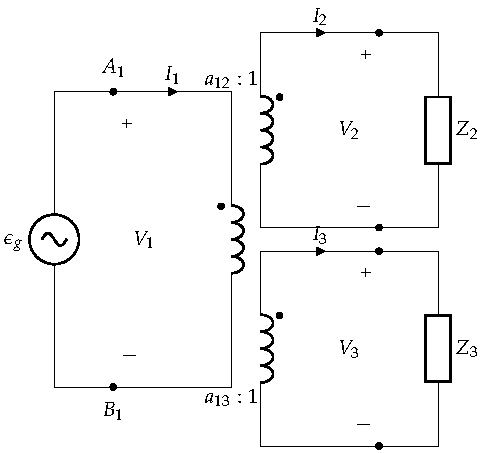
\includegraphics[height=0.9\textheight]{figs/TrafoIdealVariosDevanados_Impedancia.pdf}
\end{center}
\end{frame}


\begin{frame}[label={sec:org66ddb48}]{Impedancia de Entrada}
\begin{columns}
\begin{column}{0.4\columnwidth}
\begin{center}
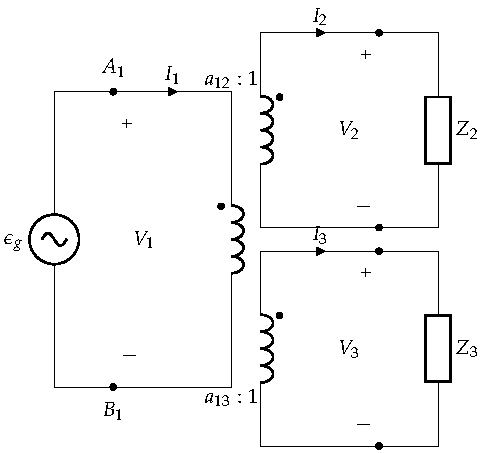
\includegraphics[width=.9\linewidth]{figs/TrafoIdealVariosDevanados_Impedancia.pdf}
\end{center}
\end{column}

\begin{column}{0.6\columnwidth}
Ecuaciones del transformador:
\begin{align*}
  \overline{U}_1 &= \overline{U}_2 \cdot a_{12}\\
  \overline{U}_1 &= \overline{U}_3 \cdot a_{13}\\
  \overline{I}_1 &= 1/a_{12} \cdot \overline{I}_2 + 1/a_{13} \cdot  \overline{I}_3
\end{align*}

Ecuaciones Terminales
\begin{align*}
  \overline{U}_2 &= \overline{Z}_2 \cdot \overline{I}_2\\
  \overline{U}_3 &= \overline{Z}_3 \cdot \overline{I}_3
\end{align*}

Resultado:
\[
  \frac{\overline{I}_1}{\overline{U}_1} = \boxed{\overline{Y}_{in} = \frac{1}{a^2_{12} \overline{Z}_2} +  \frac{1}{a^2_{13} \overline{Z}_3}}
\]
\end{column}
\end{columns}
\end{frame}

\begin{frame}[label={sec:org4b54d05}]{Circuito Equivalente}
\begin{columns}
\begin{column}{0.5\columnwidth}
\begin{center}
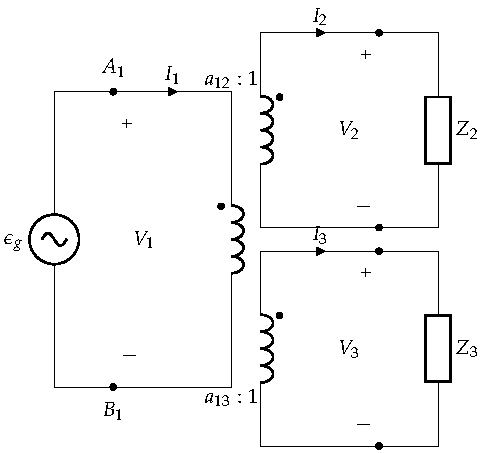
\includegraphics[width=.9\linewidth]{figs/TrafoIdealVariosDevanados_Impedancia.pdf}
\end{center}
\end{column}

\begin{column}{0.5\columnwidth}
\begin{center}
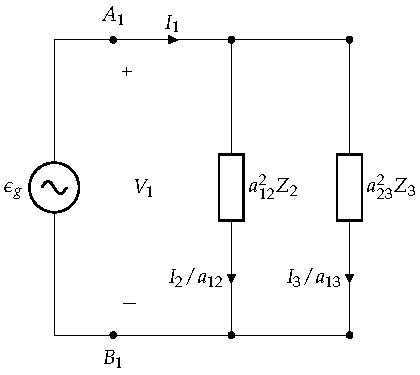
\includegraphics[width=.9\linewidth]{figs/TrafoIdealVariosDevanados_Impedancia_Equivalente.pdf}
\end{center}
\end{column}
\end{columns}
\end{frame}


\begin{frame}[label={sec:orgd00c043}]{Circuito Equivalente de un Transformador Perfecto}
\begin{columns}
\begin{column}{0.5\columnwidth}
Transformador Perfecto
\begin{center}
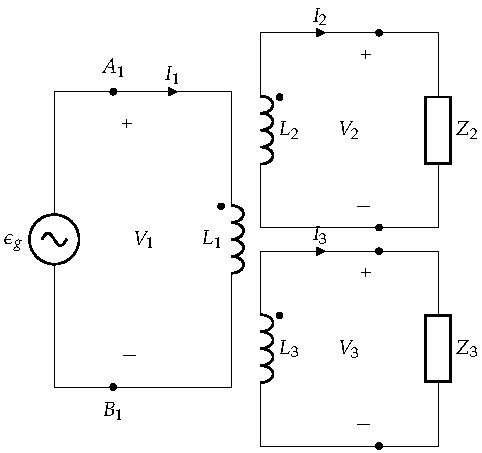
\includegraphics[width=\textwidth]{figs/TrafoPerfectoVariosDevanados_Impedancia.pdf}
\end{center}
\end{column}
\begin{column}{0.5\columnwidth}
Equivalente Ideal
\begin{center}
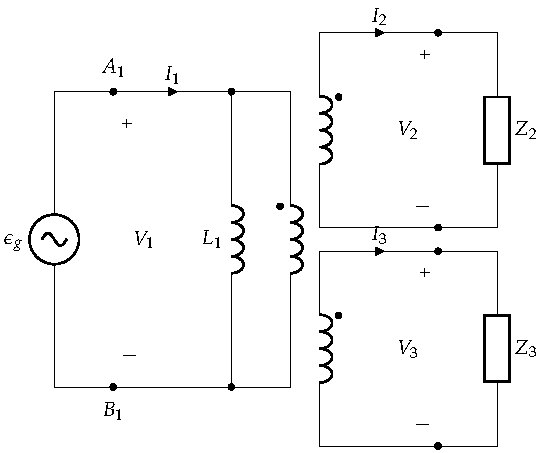
\includegraphics[width=\textwidth]{figs/TrafoPerfectoIdealVariosDevanados_Impedancia.pdf}
\end{center}
\end{column}
\end{columns}
\end{frame}

\begin{frame}[label={sec:org812aaea}]{Circuito Equivalente de un Transformador Perfecto}
\begin{columns}
\begin{column}{0.5\columnwidth}
\begin{center}
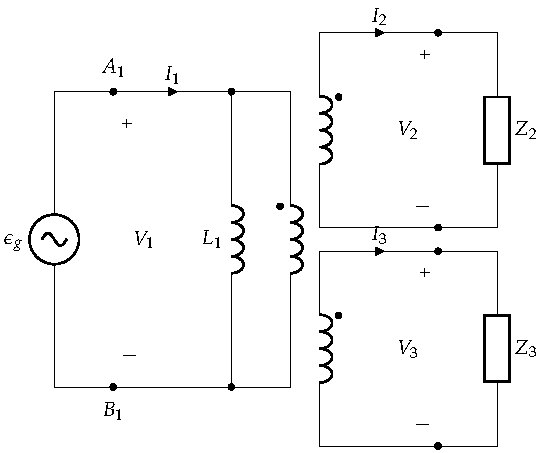
\includegraphics[width=\textwidth]{figs/TrafoPerfectoIdealVariosDevanados_Impedancia.pdf}
\end{center}
\end{column}

\begin{column}{0.5\columnwidth}
\begin{center}
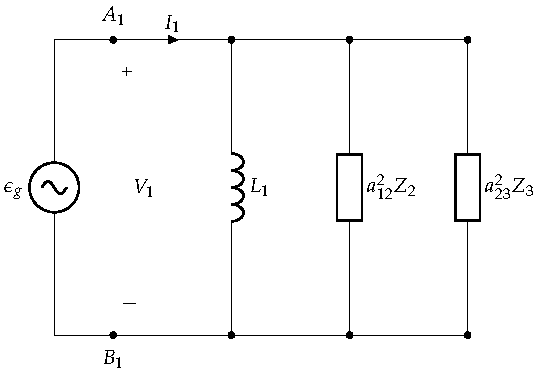
\includegraphics[width=\textwidth]{figs/TrafoPerfectoVariosDevanados_Impedancia_Equivalente.pdf}
\end{center}
\end{column}
\end{columns}
\end{frame}
\section{Autotransformador}
\label{sec:org55f6364}
\begin{frame}[label={sec:orgbec2e6e}]{Autotransformador Perfecto}
\begin{center}
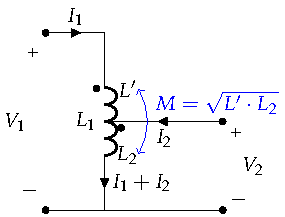
\includegraphics[height=0.9\textheight]{figs/AutotrafoPerfecto.pdf}
\end{center}
\end{frame}

\begin{frame}[label={sec:org8a09574}]{Ecuaciones del Autotransformador Perfecto}
\begin{center}
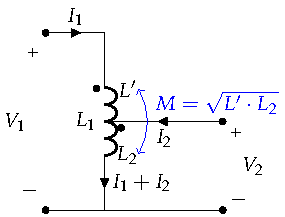
\includegraphics[height=0.5\textheight]{figs/AutotrafoPerfecto.pdf}
\end{center}

\begin{align*}
  \overline{U}_1 &= j \omega L_1 \cdot \overline{I}_1 + j \omega (M + L_2) \cdot \overline{I}_2\\
  \overline{U}_2 &= j \omega (M + L_2) \cdot \overline{I}_1 + j \omega L_2 \cdot \overline{I}_2
\end{align*}
\end{frame}
\begin{frame}[label={sec:org353c37d}]{Circuito Alternativo del Autotransformador Perfecto}
\begin{center}
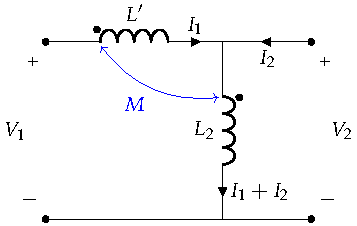
\includegraphics[width=.9\linewidth]{figs/AutotrafoPerfecto2.pdf}
\end{center}
\end{frame}

\begin{frame}[label={sec:org235db51}]{Ecuaciones del Circuito Alternativo}
\begin{center}
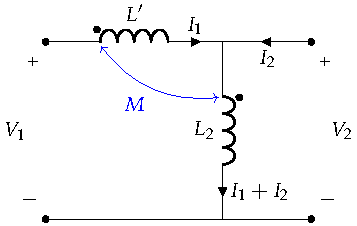
\includegraphics[height=0.5\textheight]{figs/AutotrafoPerfecto2.pdf}
\end{center}
\begin{align*}
  \overline{U}_1 &= j \omega (L' + L_2 + 2M) \cdot \overline{I}_1 + j \omega (L_2 + M) \cdot \overline{I}_2\\
  \overline{U}_2 &= j \omega (L_2 + M) \cdot \overline{I}_1 + j \omega L_2 \cdot \overline{I}_2
\end{align*}
\end{frame}

\begin{frame}[label={sec:orgcacfa1d}]{Ecuaciones Comparadas}
\begin{columns}
\begin{column}{0.4\columnwidth}
\begin{center}
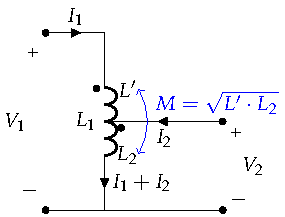
\includegraphics[height=0.4\textheight]{figs/AutotrafoPerfecto.pdf}
\end{center}
\end{column}

\begin{column}{0.6\columnwidth}
\begin{center}
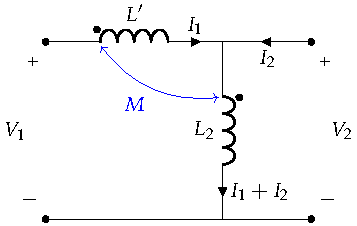
\includegraphics[height=0.4\textheight]{figs/AutotrafoPerfecto2.pdf}
\end{center}
\end{column}
\end{columns}

\begin{align*}
  \overline{U}_1 &= j \omega{\color{blue} L_1} \cdot \overline{I}_1 + j \omega{\color{red} (M + L_2)} \cdot \overline{I}_2 = j \omega{\color{blue} (L' + L_2 + 2M)} \cdot \overline{I}_1 + j \omega{\color{red} (M + L_2)} \cdot \overline{I}_2\\
  \overline{U}_2 &= j \omega{\color{red} (L_2 + M)} \cdot \overline{I}_1 + j \omega{\color{PineGreen} L_2} \cdot \overline{I}_2 = j \omega{\color{red} (L_2 + M)} \cdot \overline{I}_1 + j \omega{\color{PineGreen} L_2} \cdot \overline{I}_2
\end{align*}

\begin{align*}
  L_1 &= L' + L_2 + 2M\\
  M' &= M + L_2
\end{align*}
\end{frame}

\begin{frame}[label={sec:orgf9eb022}]{Transformador Perfecto Equivalente}
\begin{center}
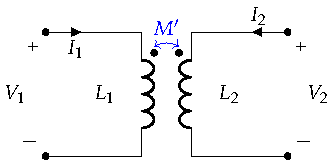
\includegraphics[height=0.6\textheight]{figs/AutoTrafo_TrafoPerfecto.pdf}
\end{center}

\begin{align*}
  L_1 &= L' + L_2 + 2M\\
  M &= \sqrt{L' \cdot L_2}\\
  M' &= M + L_2
\end{align*}
\end{frame}
\begin{frame}[label={sec:org906b343}]{Transformador Perfecto Equivalente}
\begin{center}
\includegraphics[height=0.4\textheight]{figs/AutoTrafo_TrafoPerfecto.pdf}
\end{center}
Comprobamos:
\begin{align*}
  M' &= \sqrt{L_1 \cdot L_2} = \\
     &= \sqrt{(L' + L_2 + 2M) L_2} =\\
     &= \sqrt{L'L_2 + L_2^2 + 2ML_2} =\\
     &= \sqrt{M^2 + L_2^2 + 2ML_2} = \\
     &= M + L_2
\end{align*}
\end{frame}
\begin{frame}[label={sec:org5704dc0}]{Autotransformador Ideal}
\begin{columns}
\begin{column}[b]{0.5\columnwidth}
\begin{center}
\includegraphics[width=.9\linewidth]{figs/AutoTrafoIdeal.pdf}
\end{center}
\end{column}
\begin{column}[b]{0.5\columnwidth}
\begin{center}
\includegraphics[width=.9\linewidth]{figs/Trafo_Ideal.pdf}
\end{center}
\end{column}
\end{columns}
\end{frame}
\end{document}